\subsection{Application to mouse decision-making data}
\label{sec:bestlds:results:4.3}

To asses the performance of our estimator in real-world settings, we turned to a dataset from mice performing a sensory decision-making task\footnote{Data obtained with permission directly} \cite{bolkan_opponent_2022}. In this experiment, mice ($n=13$) navigated a T-shaped maze in virtual reality. Mice were trained to detect visual cues that appeared to each side of their field of view while running down the main stem of the maze. At the end of the main stem, they had to turn toward the side of the maze with the most cues in order to receive a water reward (Figure~\ref{fig:bestlds:4}a). The mice repeated this task for many trials in a row, with an average daily session consisting of approximately 200 trials ($N=54,883$ total trials). On a random subset of $15\%$ of trials within each session, the animals' striatal dopamine D2 receptor medium spiny neurons (MSNs) were inactivated optogenetically using a 532nm laser. This transient inhibition provides a mechanism for understanding how the mice perform the task when activity in their striatum, a brain region long associated with decision-making and motor output~\cite{cox_striatal_2019, tang_differential_2022}, is suppressed. In addition to its broad association with decision-making, the striatum is the chief target of dopamine in the brain and has previously been demonstrated to encode reward prediction error signals \cite{schultz_activity_1994}. D2 MSNs in particular comprise a cell-type in the striatum that has specifically been linked with suppression of movement and constitute the first locus in what is known as the ``indirect pathway'' of the striatum (see~\cite{cox_striatal_2019} for a review).

\begin{figure*}[t!]
\centering
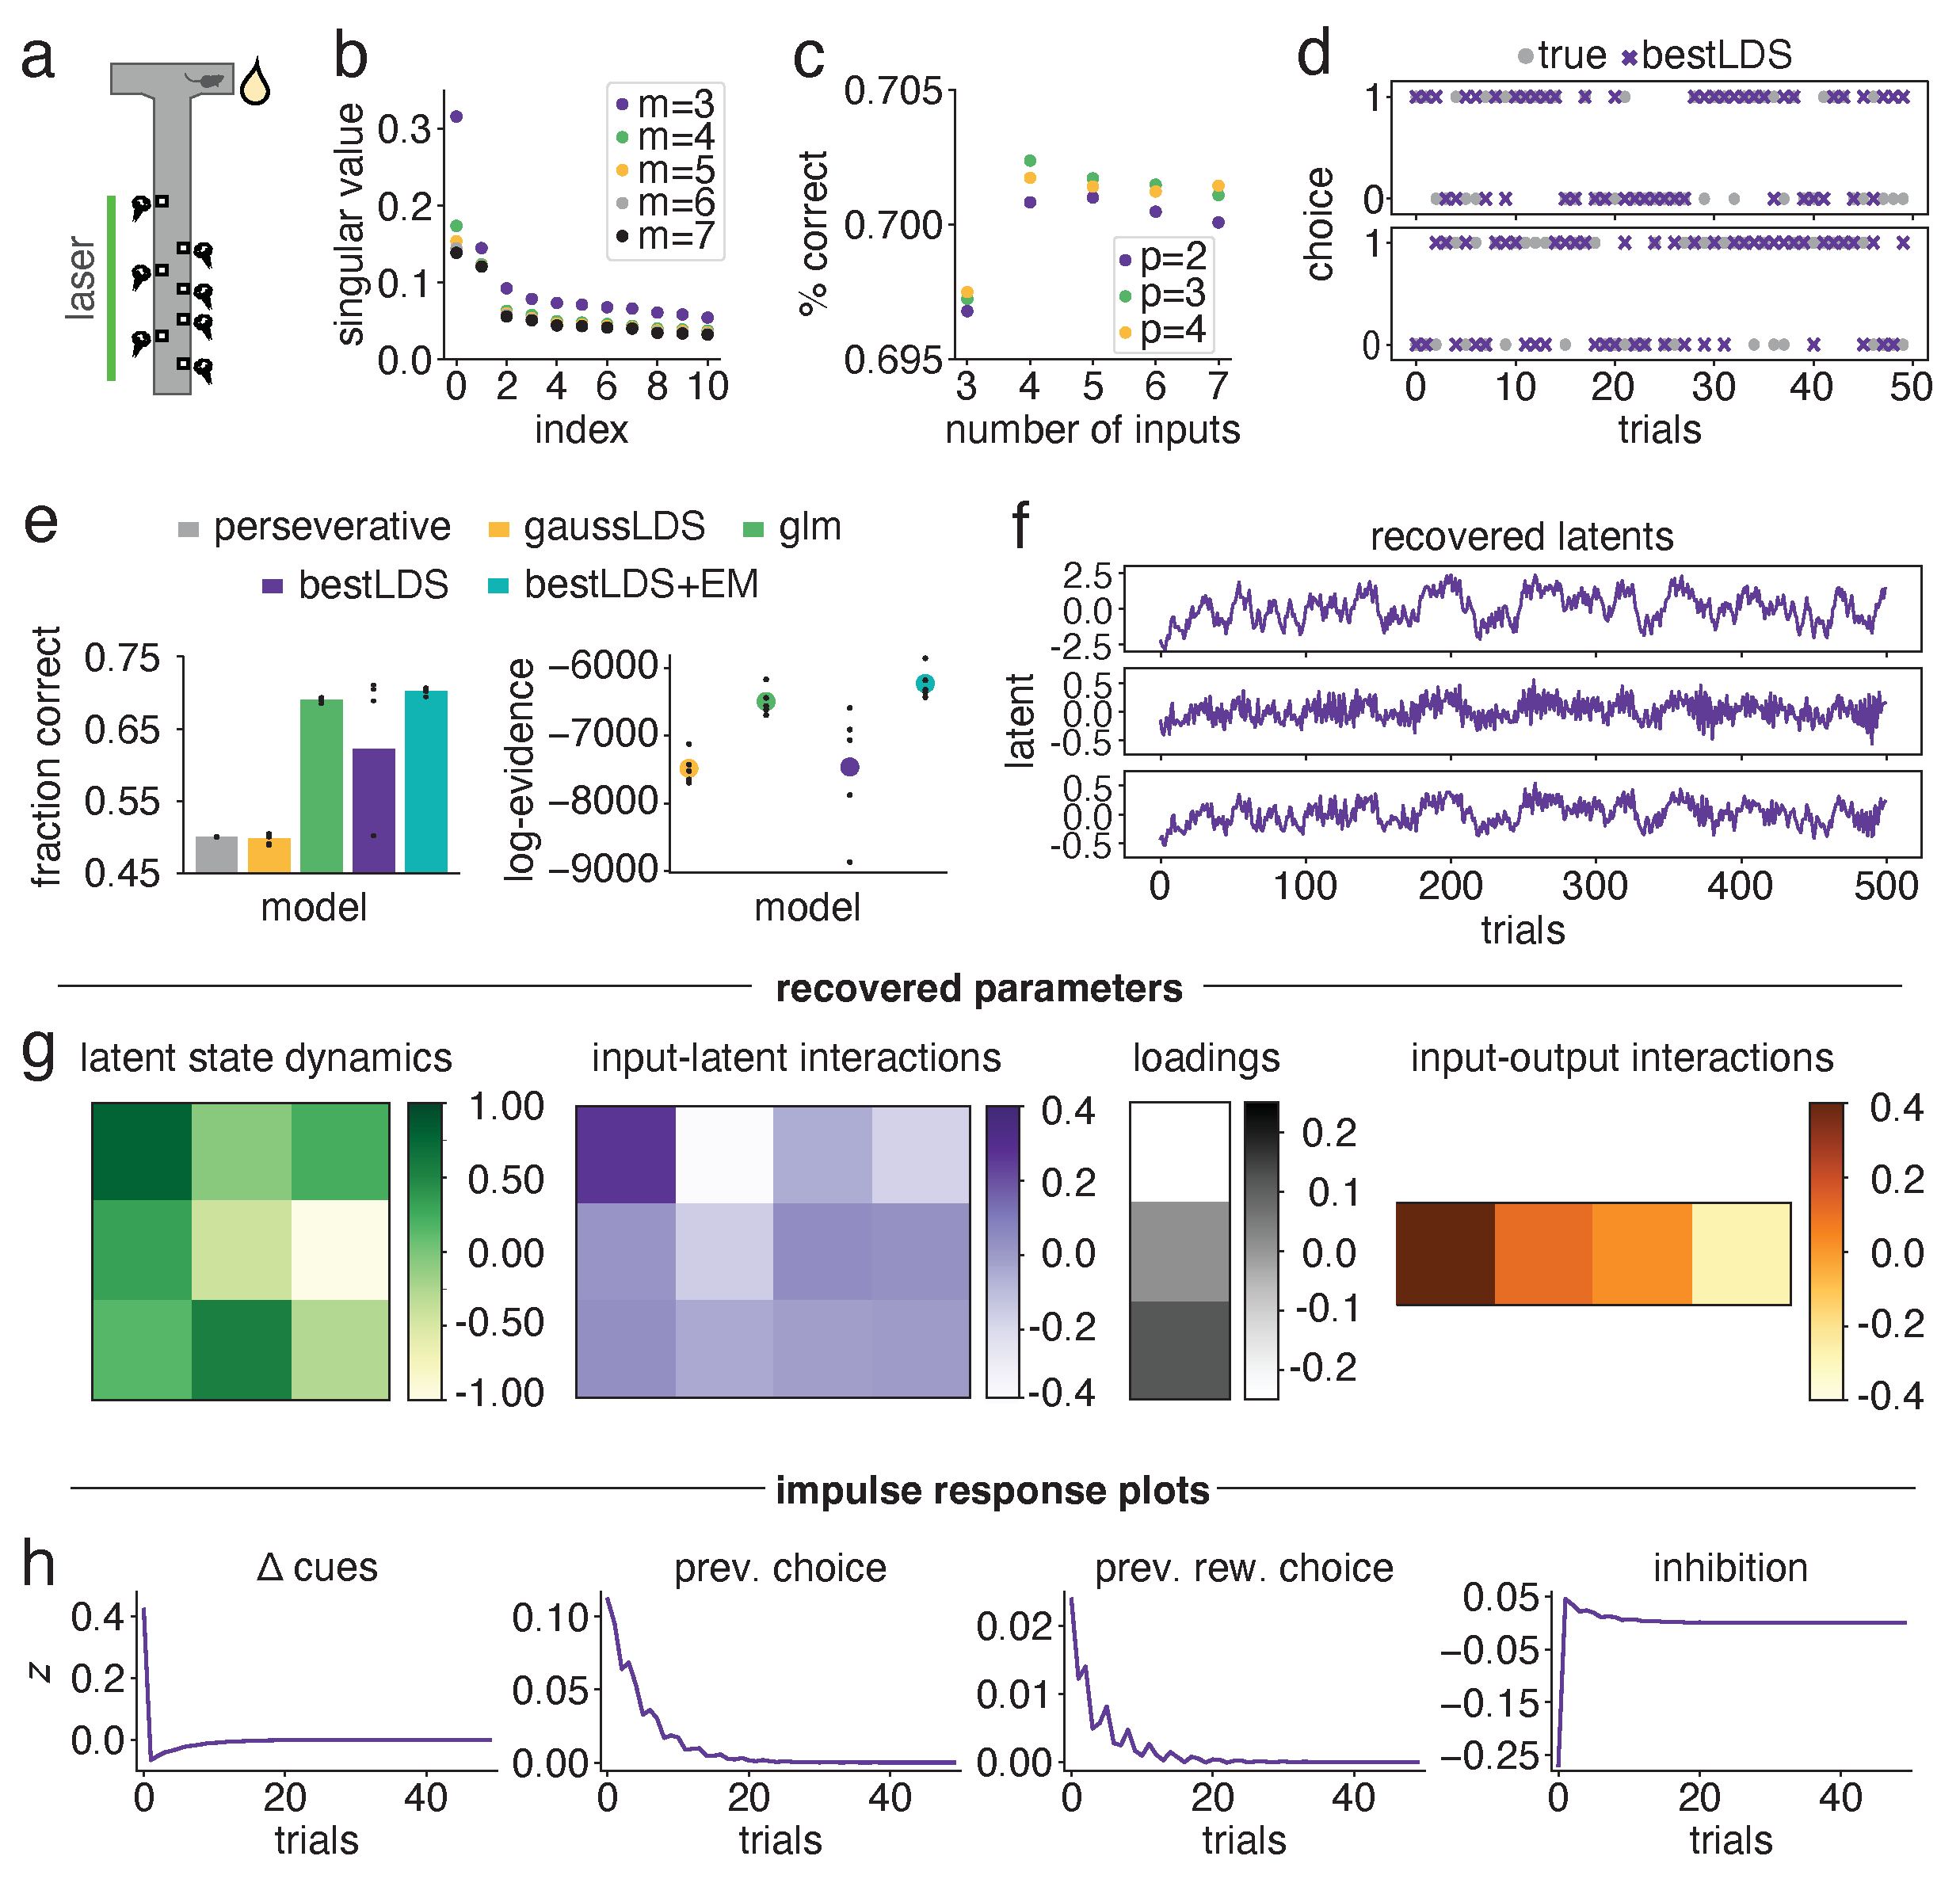
\includegraphics[width=0.90\linewidth]{ch4-bestlds/bestlds-figures/fig4.pdf}
%\vspace{-0.3cm}
\caption[Analysis of mouse binary decision-making data with bestLDS]{\textbf{Analysis of mouse binary decision-making data with bestLDS.} \textbf{(a)} Task schematic. \textbf{(b)} Singular value spectrum of the Hankel matrix with increasing number of previous choices used as inputs. \textbf{(c)} Prediction accuracy of bestLDS for various settings of $p$ and $m$. \textbf{(d)} Example stretches of predicted and true choices. \textbf{(e)} 5-fold cross-validated performance comparisons for a variety of methods on this dataset. Left: fraction of choices correctly predicted. Right: test set log-evidence. Black dots indicate each of the individual folds. \textbf{(f)} An example stretch of recovered latents. \textbf{(g)} The fitted parameters estimated by bestLDS + EM. \textbf{(h)} Impulse responses for the fitted system. In each subplot, data has been simulated noiselessly with a unit input in the indicated dimension.}
\label{fig:bestlds:4}
%\vspace{-0.4cm}
\end{figure*}

When modeling the data from this task, we take the following as inputs $u_t$ to bestLDS, given their high likelihood as relevant predictors in this task: 1) the difference between the number of right and left cues on each trial, 2) the animal's previous choice if rewarded (coded in the model as $\pm 1$ if the mouse made a correct right/left choice and 0 otherwise), and 3) the presence of inhibition (coded as $\pm 1$ if delivered to the right/left hemisphere of the brain and $0$ otherwise). We also consider including $n$-th order previous choices as additional inputs (coded as  $\pm 1$ for the right/left choice the animal made $n$ trials in the past, regardless of reward status). For our preliminary analysis, we vary the total number of previous choices incorporated in the model for $n \in \{0,1,2,3,4\}$, yielding $m \in \{3, 4, 5, 6, 7\}$. 

To determine our choice of $p$, we first examine the singular value spectrum of the transformed data (Figure~\ref{fig:bestlds:4}b). For this dataset, increasing $p$ yields only marginal decreases in the singular value after $p=4$. We correspondingly take $p=4$ as an upper-bound and conduct further analysis within the range $p \in \{2, 3, 4\}$, while also varying the number of inputs as previously described. In particular, we fit bestLDS to the data and looked at how well the inferred parameters predict subsequent choice (Figure~\ref{fig:bestlds:4}c-d) for each combination of $p$ and $m$. For all settings of $m$, the inferred parameters with $p=3$ outperform the other $p$ settings and predict choice well ($> 70\%$). Of these, the best-performing setting is with $m=4$ ($1$st-order previous choice). Therefore, for all remaining analyses we fit bestLDS with $m=4$ and $p=3$.\footnote{Note that because $q=1$, this places us in the $q<p$ regime, which can sometimes suffer from  performance issues despite performing well here; see Figure~\ref{fig:bestlds:2}.} 

It's worth noting that this approach for specifying \textit{a priori} the dimensionality of the system showcases an additional benefit of bestLDS. Without our method, the typical approach would be to fit many variants of the model using a standard inference procedure like EM, choosing the state number by some comparative method (e.g., cross-validation). However, this tends to be quite time-consuming and computationally costly. Here, the singular value spectrum combined with bestLDS fitting immediately gives an informative summary of the parameters of the dataset, providing in mere minutes what would otherwise take many hours and hundreds of different EM initializations (that is, dozens of initializations per parameter setting and value). Our spectral estimator can even be applied for this purpose when the ultimate goal is to fit to a different state-space model, such as discrete-state HMMs. 

To further assess bestLDS performance on the real data, we use five-fold cross-validation to compare its performance to three other models: a simple perseverative model, which predicts a high probability ($70\%$) of making the same choice as on the previous trial; a Gaussian LDS\footnote{We convert the real-valued observations $z$ produced by the Gaussian LDS to binary observations by taking $y_t=0$ if $z_t < \bar{z}$ and $y_t=1$ if $z_t >= \bar{z}$}; and a Bernoulli generalized linear model (GLM; Figure~\ref{fig:bestlds:4}e). Specfically, we operationalize ``performance'' in two ways: fraction of choices in the test set correctly predicted, and the log-evidence of the data evaluated under the fitted parameters. Under both metrics, bestLDS significantly outperforms the perserverative and Gaussian LDS models. Furthermore, four out of five teset sets achieve equal or greater performance than the GLM on the prediction accuracy metric, though this is not borne out in the log-evidences. This is already notable, given that bestLDS only returns an estimate of the system parameters for a multi-state LDS, whereas the GLM is a regression model that is capable of finding fairly accurate weights for a dataset of this size. However, when coupled with EM, which converges in just three steps and takes less than a minute to run, we find that the resultant estimated parameters perform better than all other methods regardless of metric.

Not only does bestLDS perform well against comparative models, but it also offers unique scientific insights into the data that don't require subsequently using the inferred parameters as EM initializations. For example, inspection of the recovered latents $x$ shows that one of the latent dimensions dominates the tendency of the overall response; the inferred traces on this latent dimension exhibit significantly higher magnitude than the other two (Figure~\ref{fig:bestlds:4}f), and the corresponding weights in the dynamics matrix $A$ are also of high magnitude (Figure~\ref{fig:bestlds:4}g, left column). As such, ``activity'' in this dimension can be described as strongly driving both the decisions of the mouse, and also the latent state of the LDS underlying it. We can examine how this is affected by the inputs by examining input-latent interactions matrix $B$; here we see that the largest magnitude elements of the matrix are those mapping the $\delta$ cues input and previous choice onto the high-magnitude dimension. Overall, this suggests that the first latent dimension is mostly driven by autocorrelation (since its self-weight in $A$ is high and the activity of the other dimensions is low), with strong influence due to the inputs, and activity in this dimension largely dominates the contribution from the latent state to the outputs.  

Furthermore, examining the input-output interactions matrix reveals the general effect that each input has on choice; more cues on the right side of the maze, a previous rightward choice, and a previous rightward rewarded choice are all more likely to elicit a rightward choice on the current trial (since they have positive weights, and right choices are coded as $1$), whereas right-hemisphere inhibition is more likely to elicit a leftward choice (since it has a negative weight). Note that the results obtained from using the bestLDS-inferred parameters as an initialization for EM produce the same qualitative interpretation of the system, indicating that for this dataset it is possible to accurately characterize the relationship between the inputs, latent states, and animals' choices solely from bestLDS without using an additional inference procedure (see Supplementary Figure~\ref{fig:ap2:4}). It's also worth noting that it would not be straightforward to reach the same conclusions by assuming linear-Gaussian observations and using standard N4SID methods. In our investigations, such an approach elicits uninterpretable system parameters, including large eigenvalues in $A$ and pathological impulse-response traces that diverge. 

A convenient way to analyze the inferred parameters is to examine their impulse responses -- that is, simulating a noiseless Bernoulli LDS with the inferred parameters starting with a unit input in a single dimension at time step $0$ (Figure~\ref{fig:bestlds:4}h). The resultant responses can be seen as a general summary of how each input affects the output state of the system -- and have been shown to be fully sufficient to characterize LTI systems. For example, a $+1$ input in the $\Delta$-cues dimension (more right cues than left) makes the system more likely to emit a right-turn, as expected given the task structure. The second trace shows that the mice perseverate (i.e., are, on average, more likely to repeat their previous action than to do the opposite one), as a previous right choice more likely causes a right turn on the current trial. The same effect holds when the previous choice was rewarded, but with smaller magnitude, suggesting that perseveration is not strongly contingent on reward. The negative response in the final trace indicates that inhibiting neural activity in one hemisphere encourages the mice to turn contralaterally (i.e., inhibition of the striatum on the right hemisphere will influence the mice to turn left). Also note the relatively long decay times for choice-related inputs, which speak to the perseverative aspect of the dynamics. These conclusions largely match previously observed patterns in this data using input-output HMMs, and the performance of bestLDS+EM in predicting choice in this dataset is similar to that found in the discrete-state case \cite{bolkan_opponent_2022}. These findings raise interesting questions about the relationship between discrete- and continuous-state models for decision-making behavior that would be a promising avenue for future study. 